\section{Problem Setup} \label{sec:problem_definition}

\begin{wrapfigure}[]{R}{0.45\linewidth}
\vspace{-6mm}
    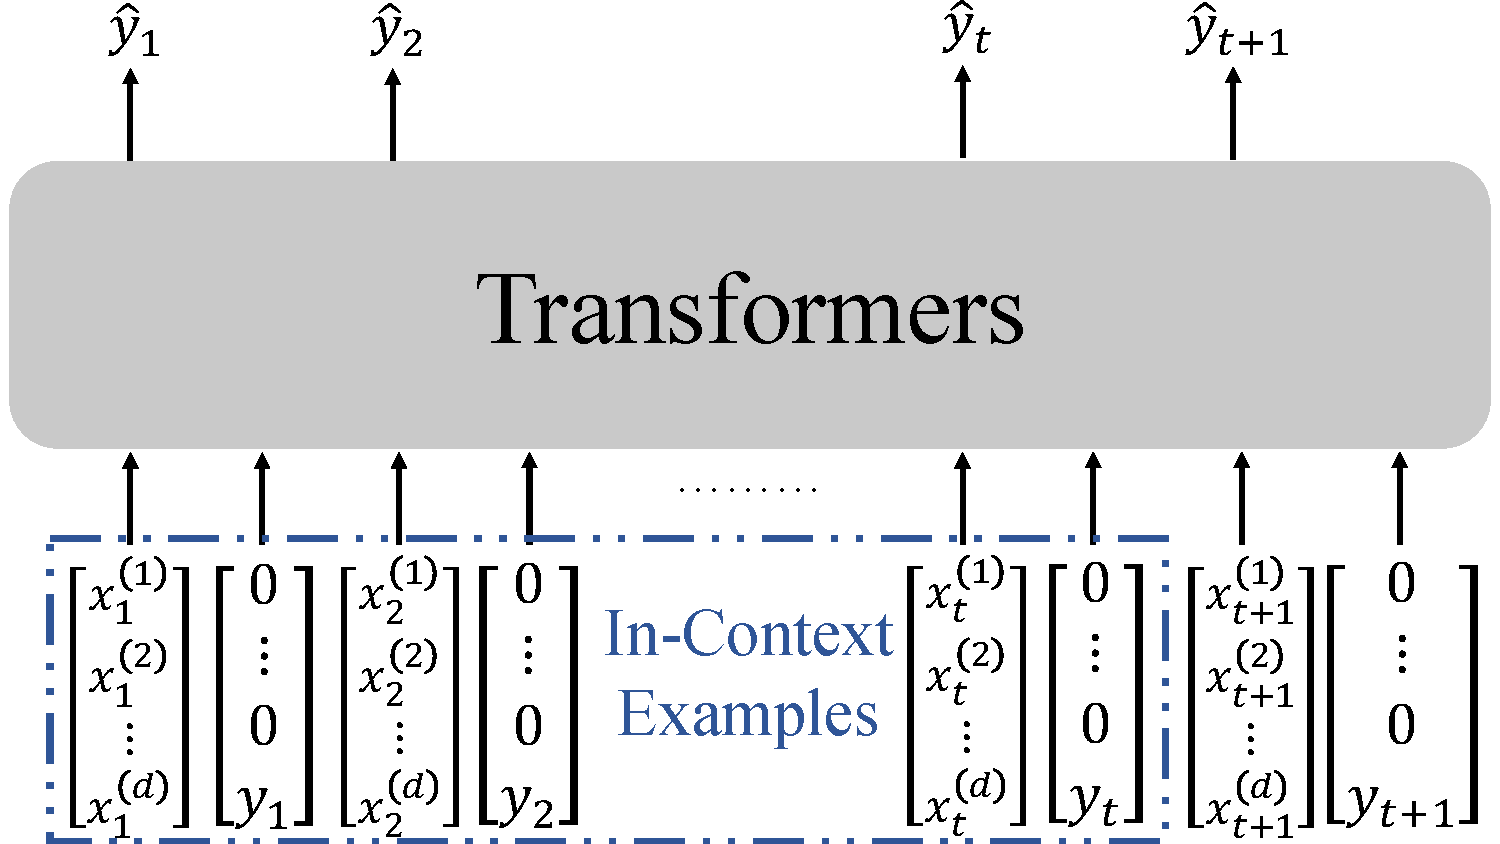
\includegraphics[width=\linewidth]{Figures/ICL.pdf}
    \captionof{figure}{Illustration of how Transformers are trained to do in-context linear regression.}
\vspace{-6mm}
\label{fig:transformer_illustration}
\end{wrapfigure}

In this paper, we  focus on the following linear regression task. The task involves $n$ examples $\{\bx_i, y_i\}_{i=1}^n$ where $\bx_i\in \R^d$ and $y_i \in \R$. The examples are generated from the following data generating distribution $P_{\mathcal{D}}$, parameterized by a distribution $\mathcal{D}$ over $(d \times d)$ positive semi-definite matrices. For each sequence of $n$ in-context examples, we first sample  a ground-truth weight vector $\bw^\star \iid \mathcal N(\zero, \bI) \in \mathbb R^d$ and a matrix $\bSigma\iid \mathcal{D}$. For $i\in [n]$, we sample each $\bx_i \iid \mathcal N(\zero, \bSigma)$. The label $y_i$ for each $\bx_i$ is given by $y_i = \bw^{\star\top} \bx_i$. Note that for much of our experiments $\mathcal{D}$ is only supported on the identity matrix $\bI$ and hence $\bSigma=\bI$, but we also consider some distributions over ill-conditioned matrices, which give rise to ill-conditioned regression problems.  Most of our results are on this noiseless setup and results with the noisy setup are in \Cref{ssec:noisy}.



\subsection{Standard Methods for Solving Linear Regression} \label{ssec:other_methods}


\new{Our central research question is:
\begin{center}
    % \textit{\textbf{Does the algorithm Transformers learn for linear regression use second-order information?}}
    \textit{\textbf{What convergence rate does the algorithm Transformers learn for linear regression achieve?}}
\end{center}}

%Is the algorithm Transformers learn for linear regression beyond first-order?



%Here we discuss various known algorithms we compare Transformers with. 
To investigate this question, we first discuss various known algorithms for linear regression. We then compare them with Transformers empirically in \S\ref{sec:experiments} and theoretically in \S\ref{sec:mechanism}, to evaluate if Transformers are more similar to first-order or second-order methods. We care particularly about algorithms' convergence rates (the number of steps required to reach an $\epsilon$ error).

For any time step $t$, let $\bX^{(t)} = \begin{bmatrix}
    \bx_1  & \cdots & \bx_t
\end{bmatrix}^\top$ be the data matrix and $\by^{(t)} = \begin{bmatrix}
    y_1 & \cdots & y_t
\end{bmatrix}^\top$ be the labels for all the datapoints seen so far. Note that since $t$ can be smaller than the data dimension $d$, $\bX^{(t)}$ can be singular.  We now consider various algorithms for making predictions for $\bx_{t+1}$ based on $\bX^{(t)}$ and $\by^{(t)}$. When it is clear from context,  we drop the superscript and refer to $\bX^{(t)}$ and $\by^{(t)}$ as $\bX$ and $\by$, where  $\bX$ and $\by$ correspond to all the datapoints seen so far.

% \begin{figure}[t]
%     \centering   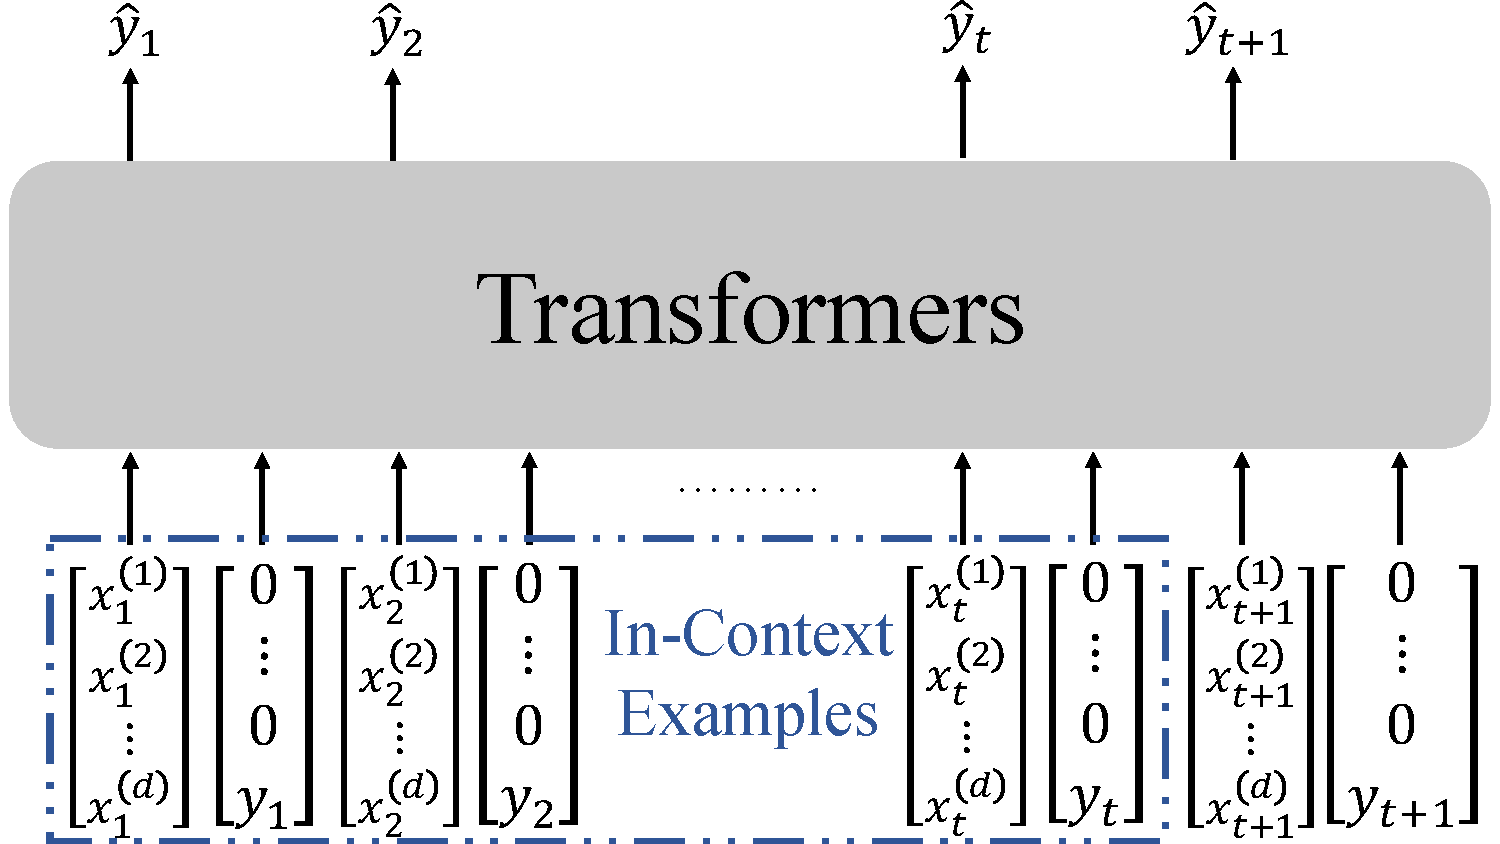
\includegraphics[width=0.75\linewidth]{Figures/ICL.pdf}
%     \caption{Illustration of how Transformers are trained to do in-context linear regression.}
%     \vspace{-1ex}
% \label{fig:transformer_illustration}
% \end{figure}
\paragraph{Ordinary Least Squares.}
This method finds the minimum-norm solution to the objective:
\begin{equation}
    \mathcal L(\bw \mid \bX, \by) = \frac{1}{2n}\|\by - \bX \bw \|_2^2.
    \label{eqn:obj}
\end{equation}
The Ordinary Least Squares (OLS) solution has a closed form given by the Normal Equations:\begin{equation}
    \hat{\bw}^\mathrm{OLS} = (\bX^\top \bX)^\dagger \bX^\top \by 
\end{equation}
where $\bS := \bX^\top \bX$  and $\bS^\dagger$ is the pseudo-inverse \citep{moonre1920pseudo} of $\bS$.

\paragraph{Gradient Descent.}  Gradient descent (GD) is a first-order method which finds the weight vector $\hat{\bw}^\mathrm{GD}$ with initialization $\hat{\bw}^\mathrm{GD}_0 = \zero$ using the iterative update rule:
\begin{equation}
\begin{aligned}
    & \hat{\bw}^\mathrm{GD}_{k+1} = \hat{\bw}^\mathrm{GD}_{k} - \eta \nabla_{\bw} \mathcal L(\hat{\bw}^\mathrm{GD}_{k} \mid \bX, \by).
\end{aligned}
\end{equation}
It is known that GD requires $\mathcal O\left(\kappa(\bS) \log(1/\epsilon)\right)$  steps to converge to an $\epsilon$ error where $\kappa(\bS) = \frac{\lambda_{\max}(\bS)}{\lambda_{\min}(\bS)}$ is the \textit{condition number}. Thus, when $\kappa(\bS)$ is large, GD converges slowly \citep{boyd2004convex}. 

\paragraph{Online Gradient Descent.}
While GD computes the gradient with respect to the full data matrix $\bX$ at each iteration, Online Gradient Descent (OGD) is an online algorithm that only computes gradients on the newly received data point $\{\bx_k, y_k\}$ at step $k$:
\begin{equation}
    \hat{\bw}^\mathrm{OGD}_{k+1} = \hat{\bw}^\mathrm{OGD}_{k} - \eta_k \nabla_{\bw} \mathcal L(\hat{\bw}^\mathrm{OGD}_{k} \mid \bx_k, y_k).
\end{equation}
Picking $\eta_k = \frac{1}{\|\bx_k\|_2^2}$ ensures that the new weight vector $\hat{\bw}^\mathrm{OGD}_{k+1}$ makes zero error on $\{\bx_k, y_k\}$. 


\paragraph{\newton's Method.} This is a second-order method which finds the weight vector $ \hat{\bw}^\mathrm{Newton}$ by iteratively apply Newton's method to finding the pseudo inverse of $\bS = \bX^\top \bX$ \citep{schulz1933inverse,adi1965ai}. 
\begin{equation}
    \begin{aligned}
        &\bM_0 = \alpha \bS \textrm{, where } \alpha = \frac{2}{\|\bS \bS^\top\|_2 }, ~~ \hat{\bw}^\mathrm{Newton}_0 = \bM_0 \bX^\top \by, \\
        & \bM_{k+1} = 2 \bM_{k} - \bM_k \bS \bM_k, ~~ \hat{\bw}^\mathrm{Newton}_{k+1} =  \bM_{k+1}  \bX^\top \by. 
    \end{aligned}
\end{equation}
This computes an approximation of the  psuedo inverse using the moments of $\bS$. In contrast to GD, the \newton's method only requires $\mathcal O(\log \kappa(\bS) + \log \log (1/\epsilon))$ steps to converge to an $\epsilon$ error \citep{soderstrom1974onp,Pan1991AnIN}. Note that this is exponentially faster than the convergence rate of GD. %Note that this is equivalent to computing a Taylor series approximation of the psuedo inverse using the moments of $\bS$.
We discuss additional algorithms such as Conjugate Gradient, BFGS, and L-BFGS in the Appendix \ref{sec:second-order}.

\vspace{-1mm}
\subsection{Solving Linear Regression with Transformers}
\vspace{-1mm}

We will use neural network models such as Transformers to solve this linear regression task. As shown in \Cref{fig:transformer_illustration}, at time step $t+1$, the model sees the first $t$ in-context examples $\{\bx_i,y_i\}_{i=1}^t$, and then makes predictions for $\bx_{t+1}$, whose label $y_{t+1}$ is not observed by the Transformers model.

We randomly initialize our models and then train them on the linear regression task to make predictions for every number of in-context examples $t$, where $t\in [n]$. Training and test data are both drawn from $P_{\mathcal{D}}$. To make the input prompts contain both $\bx_i$ and $y_i$,  we follow same the setup as \citet{Garg2022WhatCT}'s to zero-pad $y_i$'s, and use the same GPT-2 model \citep{radford2019language} with softmax activation and causal attention mask  (discussed later in \cref{def:attn}). 

We now present the key mathematical details for the Transformer architecture, and how  they can be used for in-context learning.
First, the causal attention mask enforces that attention heads can only attend to hidden states of previous time steps, and is defined as follows.


\begin{definition}[Causal Attention Layer]\label{def:attn}
    A \textbf{causal} attention layer with $M$ heads and activation function $\sigma$  is denoted as $\mathrm{Attn}$ on any input sequence $\bH = \begin{bmatrix}
        \bh_1, \cdots, \bh_N
    \end{bmatrix} \in \mathbb R^{D \times N}$, where $D$ is the dimension of hidden states and $N$ is the sequence length. In the vector form,
    \begin{equation}
        \tilde{\bh}_t = [\mathrm{Attn}(\bH)]_t = \bh_t +  \sum_{m=1}^M \sum_{j=1}^t \sigma \left(\inner{\bQ_m \bh_t, \bK_m \bh_j}\right) \cdot \bV_m \bh_j.
    \end{equation}
\end{definition}
\citet{Vaswani2017AttentionIA} originally proposed the Transformer architecture with the Softmax activation function for the attention layers. Later works have found that replacing $\mathrm{Softmax}(\cdot)$ with $\frac{1}{t} \mathrm{ReLU}(\cdot)$ does not hurt model performance \citep{Cai2022EfficientViTEL,shen2023study,wortsman2023replacing}. The Transformers architecture is defined by putting together attention layers with feed forward layers: 



\begin{definition}[Transformers]
    An $L$-layer decoder-based transformer with Causal Attention Layers is denoted as $\mathrm{TF}_{\btheta}$ and is a composition of a MLP Layer (with a skip connection) and a Causal Attention Layers. For input sequence $\bH^{(0)}$, the transformers $\ell$-th hidden layer is given by
    \begin{equation}
      \mathrm{TF}_{\btheta}^{\ell}(\bH^{(0)}) :=  \bH^{(\ell)} = \mathrm{MLP}_{\btheta_\mathrm{mlp}^{(\ell)}} \left(\mathrm{Attn}_{\btheta_\mathrm{attn}^{(\ell)}} (\bH^{(\ell-1)})\right). \nonumber
    \end{equation}
    where $\btheta = \{\btheta_\mathrm{mlp}^{(\ell)}, \btheta_\mathrm{attn}^{(\ell)}\}_{\ell=1}^L$ and $\btheta_\mathrm{attn}^{(\ell)} = \{\bQ_m^{(\ell)}, \bK_m^{(\ell)}, \bV_m^{(\ell)}\}_{m=1}^M$ has $M$ heads at layer $\ell$. 
\label{def:transformers}
\end{definition}

In particular for the linear regression task, Transformers perform in-context learning as follows
\begin{definition}[Transformers for Linear Regression] \label{def:readout}
Given in-context examples $\{\bx_1, y_1, \dotsc, \bx_t, y_t\}$, Transformers make predictions on a query example $\bx_{t+1}$  through a readout layer parameterized as $\btheta_{\mathrm{readout}} = \{\bu, v\}$, and the prediction $\hat{y}_{t+1}^{\mathrm{TF}} $ is given by
\begin{align*}
    \hat{y}_{t+1}^{\mathrm{TF}} &:= \mathrm{ReadOut} \Big[\underbrace{\mathrm{TF}_{\btheta}^L (\{\bx_1, \by_1, \cdots, \bx_t, \by_t, \bx_{t+1}\})}_{\bH^{(L)}} \Big] = \bu^\top \bH^{(L)}_{:,2t+1} + v.
\end{align*}
\end{definition}

\new{To compare the rate of convergence of iterative algorithms to that of Transformers, we treat the layer index $\ell$ of Transformers as analogous to the iterative step $k$ of algorithms discussed in \S \ref{ssec:other_methods}. Note that for Transformers, we need to re-train the $\mathrm{ReadOut}$ layer for every layer index $\ell$ so that they can improve progressively (see \S\ref{ssec:progress} and for experimental details) for linear regression tasks.}

% \subsection{LSTM}
% While our primary goal is to analyze Transformers, we also consider LSTMs \citep{hochreiter1997lstm} to understand whether Transformers learn different algorithms than other neural sequence models trained to do linear regression. In particular, we train a unidirectional $L$-layer LSTM, which generates a sequence of hidden states $\bH^{(\ell)}$ for each layer $\ell$, similarly to an $L$-layer Transformer.
% As with Transformers, we add a readout layer that predicts the $\hat{y}_{t+1}^{\mathrm{LSTM}}$ from the final hidden state at the final layer, $\bH_{:,2t+1}^{(L)}$.
\begin{figure*}[t]
    \centering
    \subfigure[Transformers]{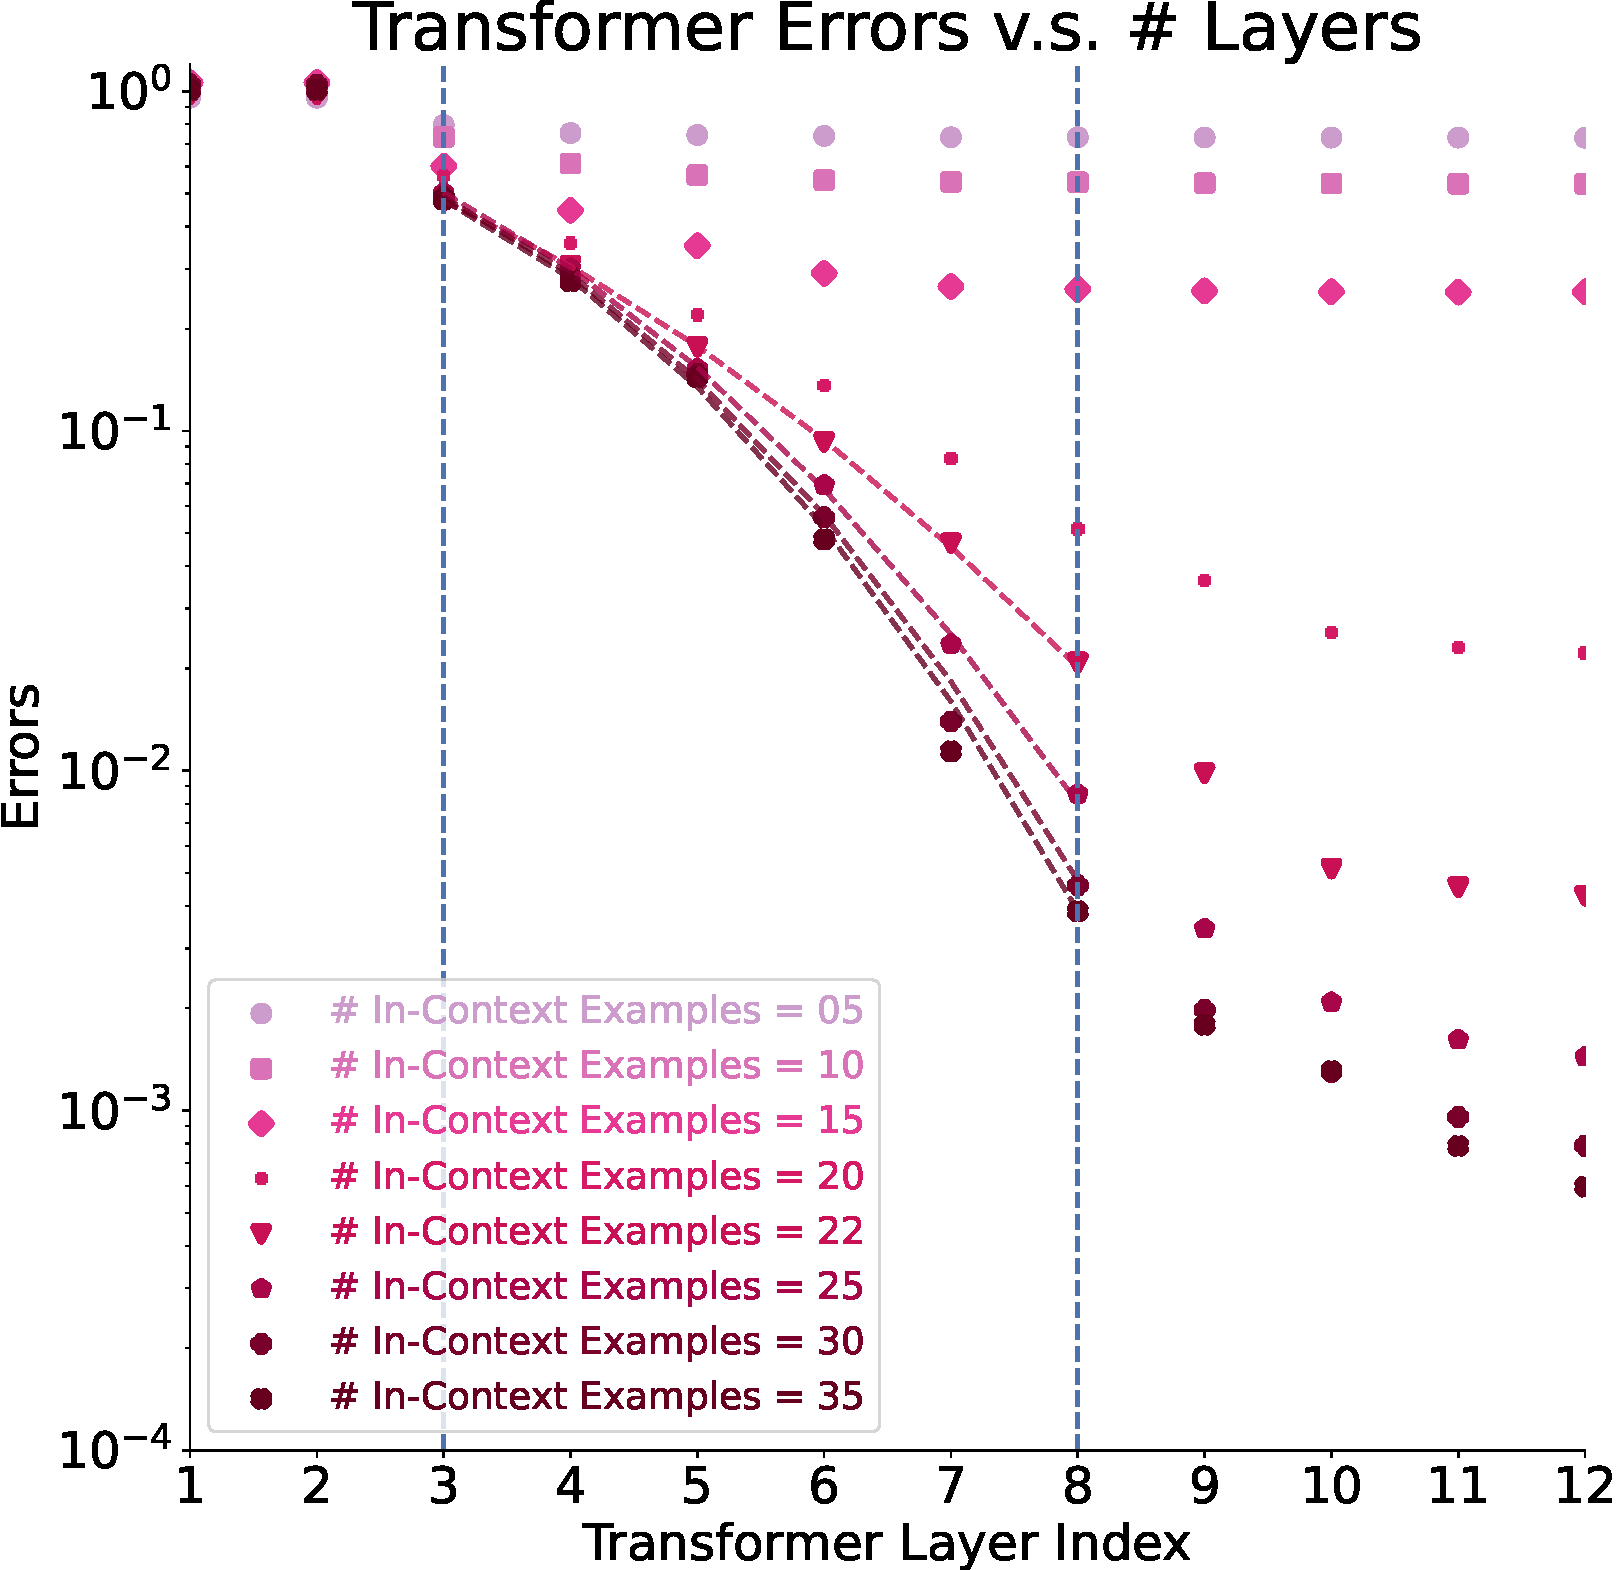
\includegraphics[width=0.315\linewidth]{Figures/convergence/transformers_convergence.pdf} \label{subfig:transformers-convergence} } 
    \subfigure[Iterative Newton's Method]{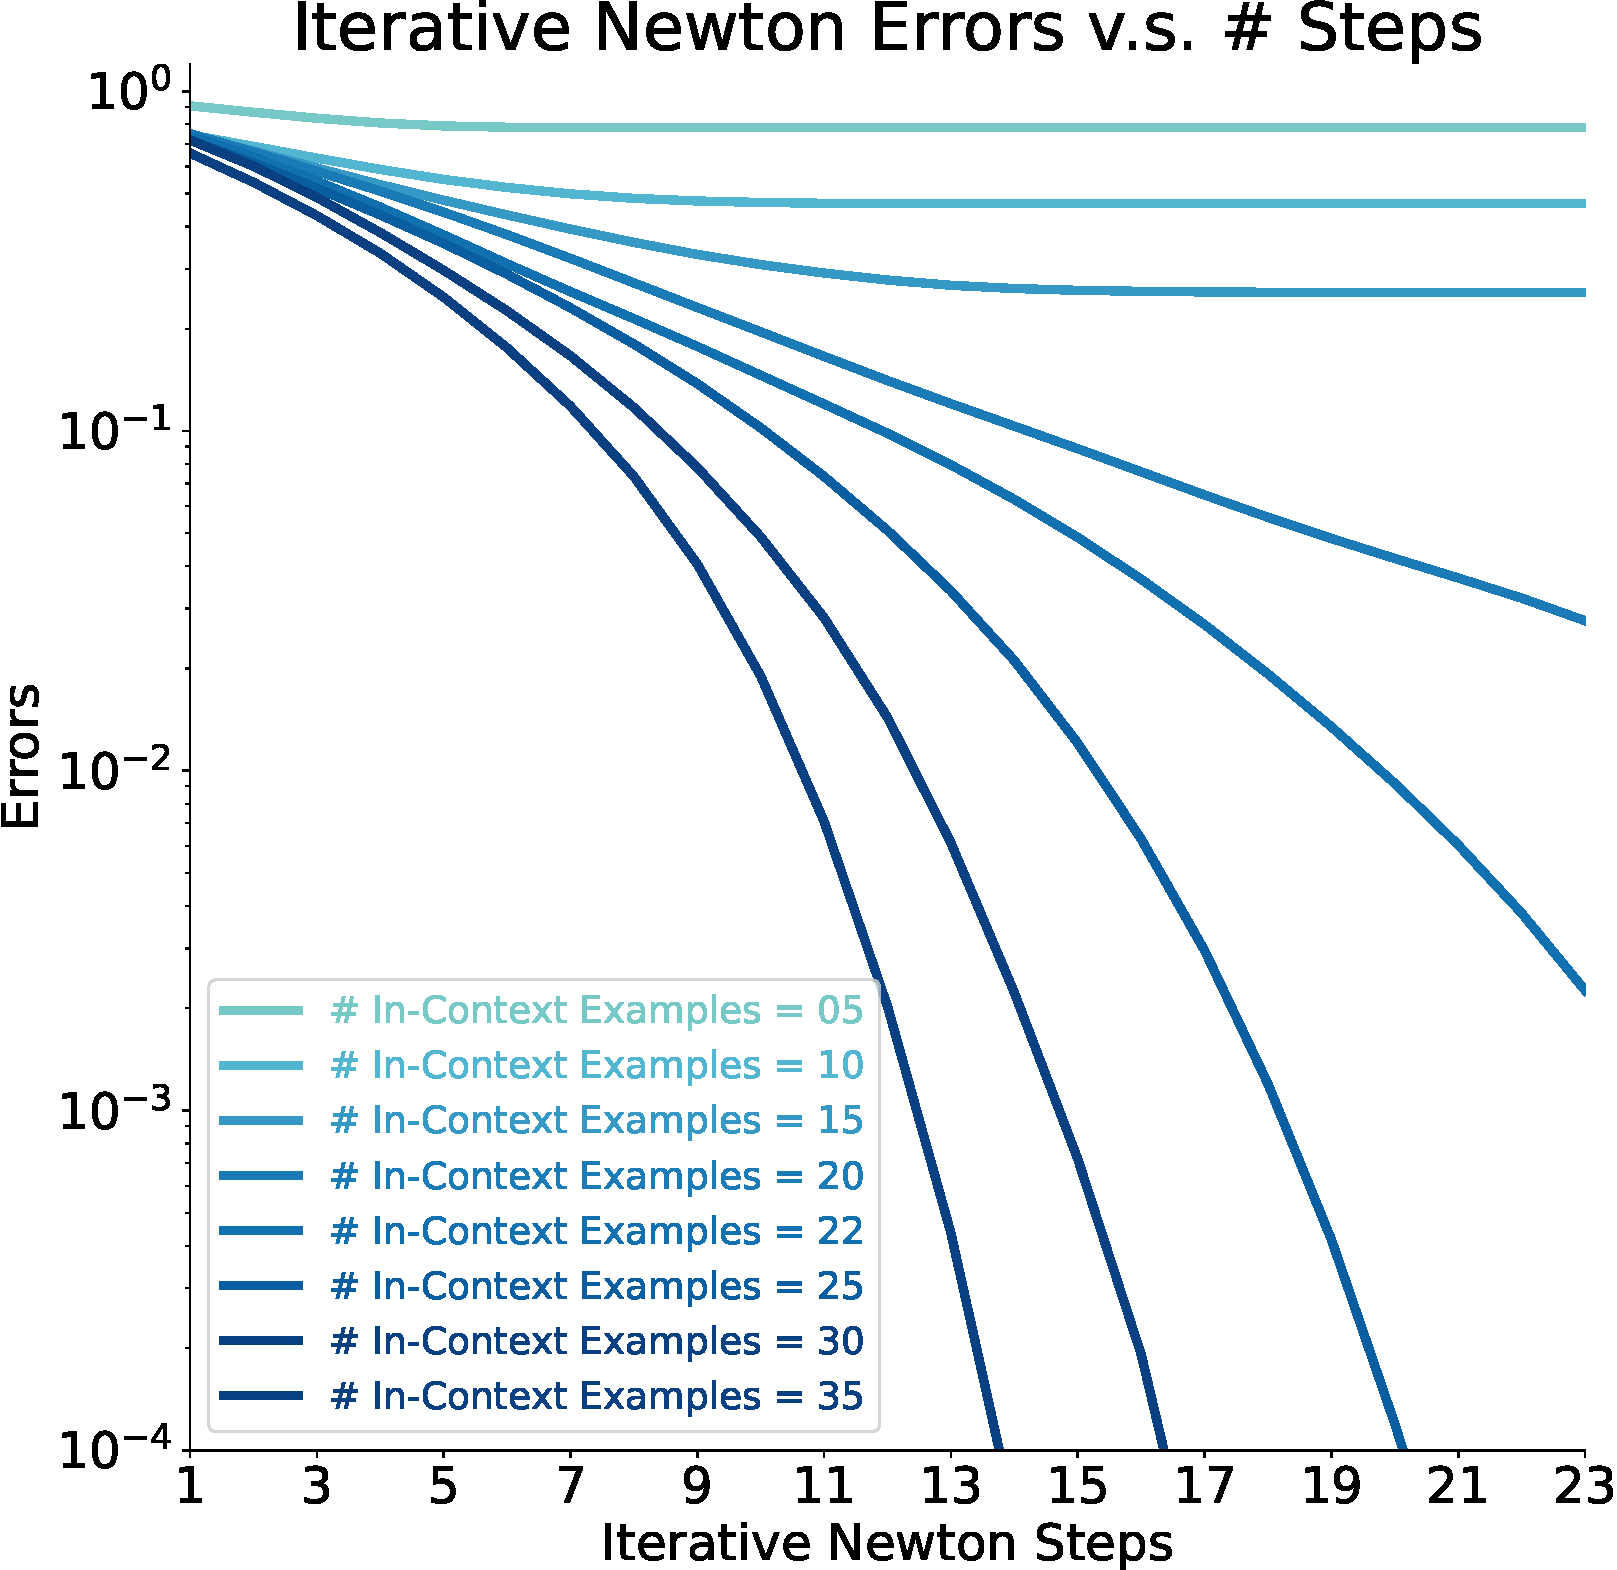
\includegraphics[width=0.315\linewidth]{Figures/convergence/newton_convergence.pdf} \label{subfig:newton-convergence} } 
    \subfigure[Gradient Descent]{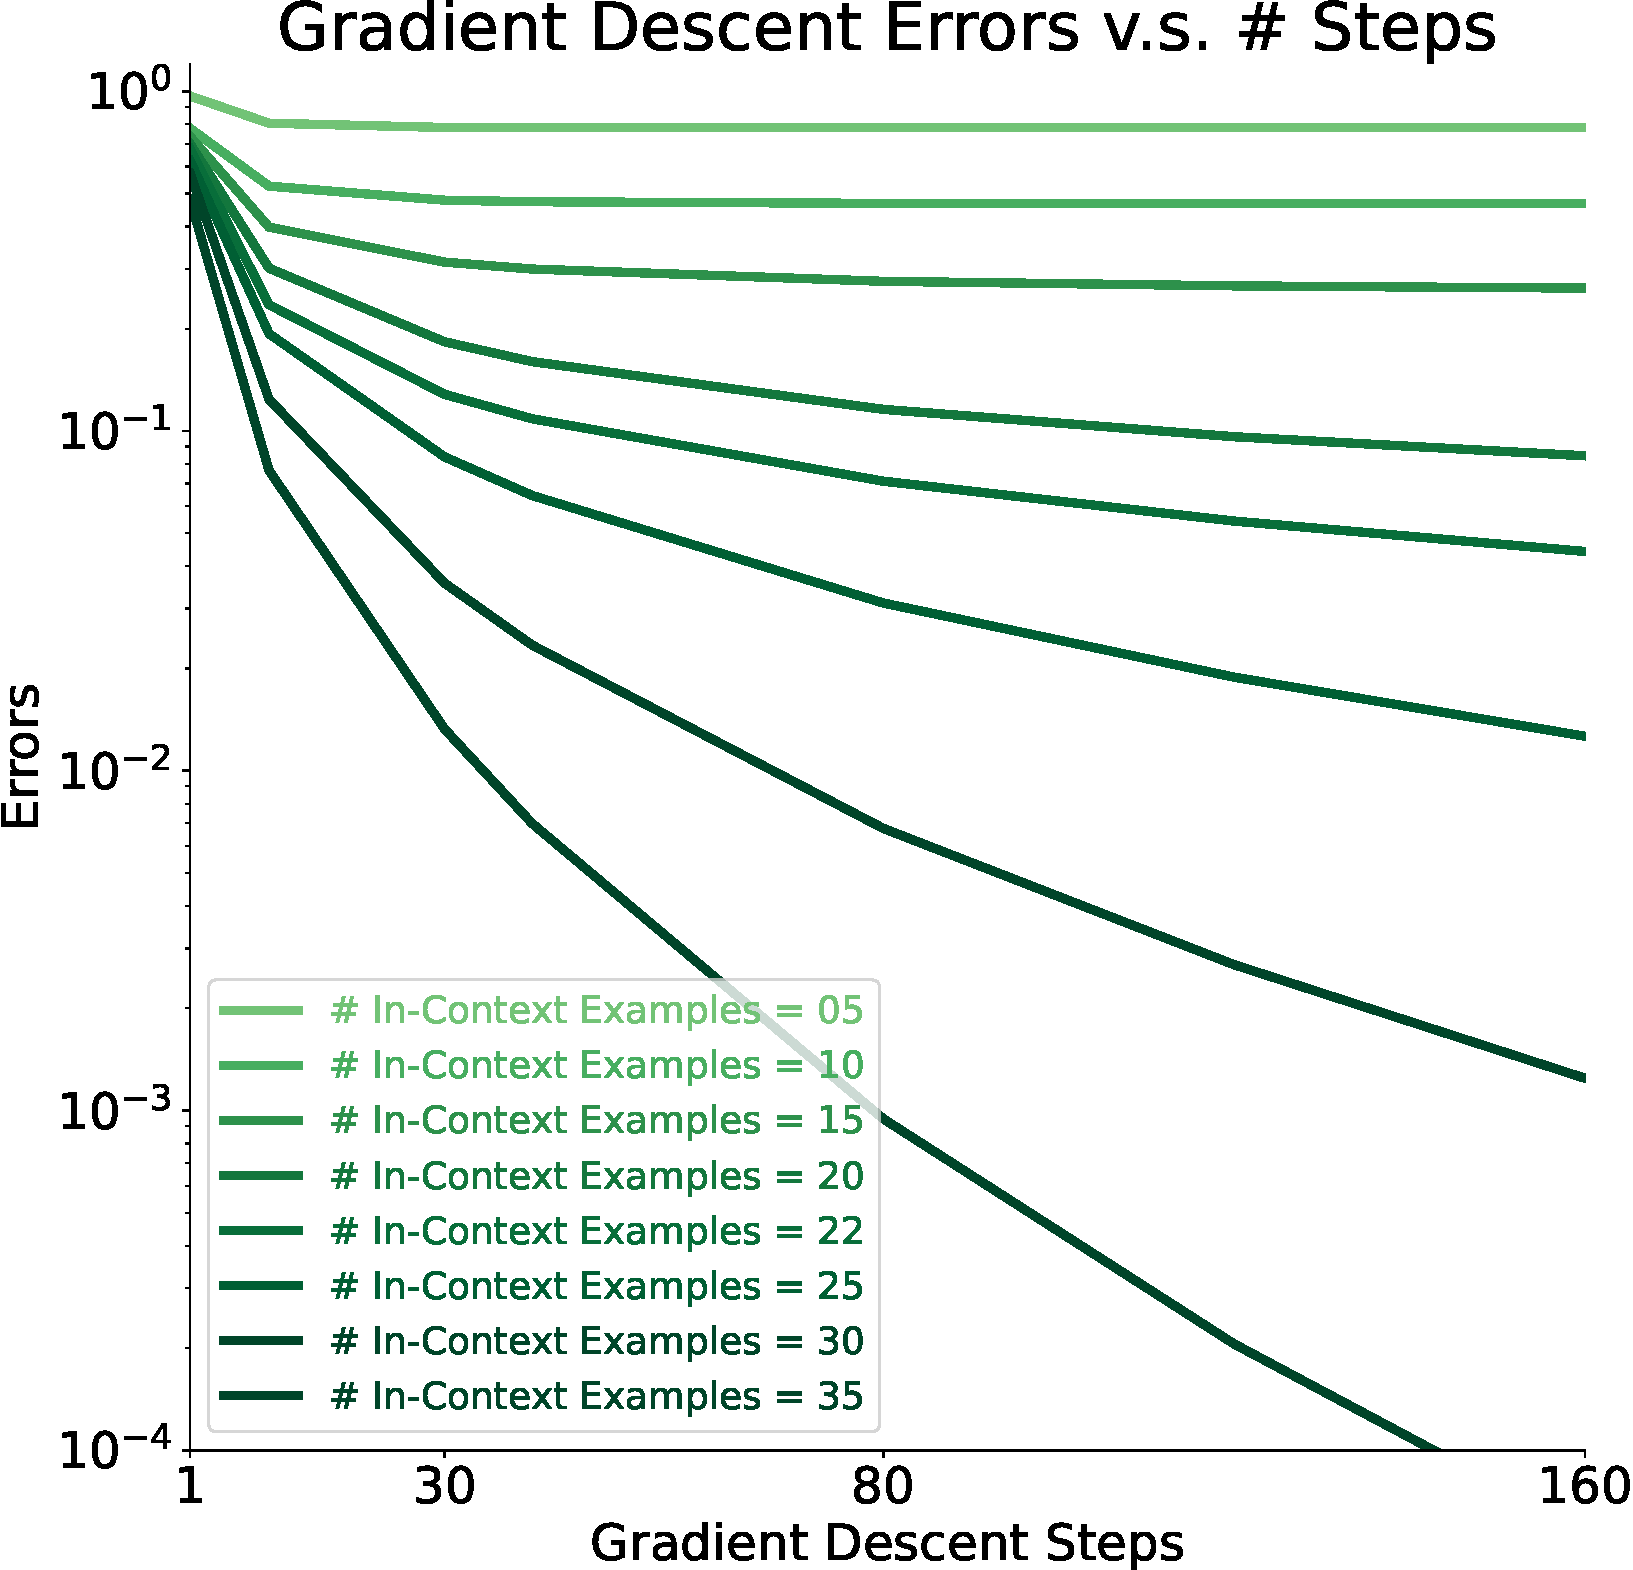
\includegraphics[width=0.315\linewidth]{Figures/convergence/gd_convergence.pdf} \label{subfig:gd-convergence}} 
    \caption{\textbf{Convergence of Algorithms. Similar to \newton\ and GD, Transformer's performance improve over the layer index $\ell$. When $n > d$, the Transformer model, from layers 3 to 8, demonstrates a superlinear convergence rate, similar to \newton, while GD, with fixed step size, is sublinear. Later layers of Transformers show a slower convergence rate, and we hypothesize they have little incentive to implement the algorithm precisely since the error is already very small. A 24-layer Transformer model exhibits the same superlinear convergence (\Cref{fig:convergence-24layer} in \S\ref{app:24-layer}).}}
    \vspace{-1.5ex}
    \label{fig:convergence}
\end{figure*}

\vspace{-1mm}
\subsection{Measuring Algorithmic Similarity}
\vspace{-1mm}

%\subsubsection{Metrics} \label{ssec:metric}
We propose two metrics to measure the similarity between linear regression algorithms.

\paragraph{Similarity of Errors.} This metric aims to measure similarity of algorithms through comparing prediction errors. For a linear regression algorithm $\calA$,
let $ \calA(\bx_{t+1} \mid \{\bx_i, y_i\}_{i=1}^{t})$ 
denote its prediction on the $(t+1)$-th in-context example $\bx_{t+1}$ after observing the first $t$ examples (see \Cref{fig:transformer_illustration}). 
We write $\calA(\bx_{t+1}) := \calA(\bx_{t+1} \mid \{\bx_i, y_i\}_{i=1}^{t})$ for brevity. Errors (i.e., residuals) on the sequence are:\footnote{the indices start from 2 to $n+1$ because we evaluate all cases where $t$ can choose from $1,\cdots, n$.}
\begin{equation}
    \calE(\calA \mid \{\bx_i, y_i\}_{i=1}^{n+1}) = \Big[
        \calA(\bx_{2}) - y_2 ,\cdots, \calA(\bx_{n+1}) - y_{n+1}
   \Big]^\top. \nonumber
\end{equation}
%\tianqi{I wonder why the index starts from 2?}
The similarity of errors for two algorithms $\calA_a$ and $\calA_b$ is the expected cosine similarity of their errors on a randomly sampled data sequence:
\begin{equation*}
    \mathrm{SimE}(\calA_a, \calA_b) 
    =   \mathop{\mathbb E}_{\{\bx_i, y_i\}_{i=1}^{n+1} \sim P_{\mathcal{D}}} \Bigg[
    \calC\Big(\calE(\calA_a | \{\bx_i, y_i\}_{i=1}^{n+1}), 
    \calE(\calA_b | \{\bx_i, y_i\}_{i=1}^{n+1})\Big)\Bigg]. 
\end{equation*}

Here $\calC(\bu, \bv) = \frac{
    \inner{\bu, \bv}
    }{\|\bu\|_2 \|\bv\|_2}$ is the cosine similarity, $n$ is the total number of in-context examples, and $P_{\mathcal{D}}$ is the data generation process discussed previously. 

\paragraph{Similarity of Induced Weights.}
All standard algorithms for linear regression estimate a weight vector $\hat{\bw}$. 
While neural ICL models like Transformers do not explicitly learn such a weight vector, similar to \citet{Akyrek2022WhatLA},
we can \emph{induce} an implicit weight vector $\tilde{\bw}$ learned by any algorithm $\calA$ by fitting a weight vector to its predictions.
We can then measure similarity of algorithms by comparing the induced $\tilde{\bw}$.
To do this, for any fixed sequence of $t$ in-context examples  $\{\bx_i, y_i\}_{i=1}^{t}$, we sample $T\gg d$ query examples  $\tilde{\bx}_{k} \iid \mathcal N(\zero, \bSigma)$, where $k\in [T]$. For this fixed sequence of in-context examples $\{\bx_i, y_i\}_{i=1}^{t}$, we create $T$ in-context prediction tasks and use the algorithm $\calA$ to make predictions $\calA(\tilde{\bx}_k \mid \{\bx_i, y_i\}_{i=1}^{t})$. We define the induced data matrix and labels as 
\begin{equation}
    \tilde{\bX} = \begin{bmatrix}
        \tilde{\bx}_1^\top \\  \vdots \\ \tilde{\bx}_T^\top
    \end{bmatrix}  \qquad \tilde{\bY} = \begin{bmatrix}
        \calA(\tilde{\bx}_1 \mid \{\bx_i, y_i\}_{i=1}^{t}) \\ 
        \vdots \\ 
        \calA(\tilde{\bx}_T \mid \{\bx_i, y_i\}_{i=1}^{t})
    \end{bmatrix}.
\end{equation}
The induced weight vector for $\calA$ and these $t$ examples is:
\begin{equation}
    \tilde{\bw}_t(\calA) := \tilde{\bw}_t(\calA \mid \{\bx_i, y_i\}_{i=1}^t) = (\tilde{\bX}^\top \tilde{\bX})^{-1} \tilde{\bX}^\top \tilde{\bY}.
\end{equation}
% We measure the similarity between two algorithms $\calA_a$ and $\calA_b$ by measuring the similarity of induced weight vectors $\tilde{\bw}_t(\calA_a)$ and $\tilde{\bw}_t(\calA_b)$. We define the similarity of induced weights between two algorithms as the expected average cosine similarity of induced weights over all possible number of in-context data, on a randomly sampled data sequence:
The similarity of induced weights between two algorithms $\calA_a$ and $\calA_b$ is the expected average cosine similarity\footnote{Alternative metrics such as $\ell_2$ distance gives the same observation. Here cosine similarity is better since errors usually have small magnitudes, and directions of induced weights are meaningful.} of induced weights $\tilde{\bw}_t(\calA_a)$ and $\tilde{\bw}_t(\calA_b)$ over all possible $1 \leq t \leq n$, on a randomly sampled data sequence:
\begin{equation*}
    \mathrm{SimW}(\calA_a, \calA_b) =  \mathop{\mathbb E}_{\{\bx_i, y_i\}_{i=1}^{n} \sim P_{\mathcal{D}}} \Bigg[
    \frac{1}{n} \sum_{t=1}^n
    \calC\Big(\tilde{\bw}_t(\calA_a | \{\bx_i, y_i\}_{i=1}^t), \tilde{\bw}_t(\calA_b | \{\bx_i, y_i\}_{i=1}^t))\Big)\Bigg].
\end{equation*}


%\subsubsection{Best Matching Hyper-parameters Between Algorithms}

\paragraph{Matching steps between algorithms.} Each algorithm converges to its predictions after several \textbf{steps} --- for example the number of iterations for \newton\ and GD, and  the number of layers for Transformers (see \Cref{ssec:progress}). 
When comparing two algorithms, given a choice of steps for the first algorithm, we match it with the steps for the second algorithm that maximize similarity. 
\begin{definition}[Best-matching Steps] Let $\mathcal M$ be the metric for evaluating similarities between two algorithms $\calA_a$ and $\calA_b$, which have steps $p_a \in [0, T_a]$ and $p_b \in [0, T_b]$, respectively. For a given choice of $p_a$, we define the best-matching number of steps of algorithm $\calA_b$ for $\calA_a$ as: 
\begin{equation}
    p_b^{\mathcal M}(p_a) := \argmax_{p_b \in [0, T_b]} \mathcal M(\calA_a(\cdot \mid p_a), \calA_b(\cdot \mid p_b)).
\end{equation} 
\vspace{-3.4mm}
\label{def:matching}
\end{definition}
In our experiments, we chose $T_a, T_b$ be large enough integers so the algorithms converge. The matching processes can be visualized as heatmaps as shown in \Cref{fig:heatmap}, where best-matching steps are highlighted. This enables us to compare the rate of convergence of algorithms. 
In particular, if two algorithms converge at the same rate, the best matching steps between the two algorithms should follow a linear trend.
We will discuss these results in \S\ref{sec:experiments}. See \Cref{fig:best-matching} on how best-matching steps help compare the convergence rates.
